\section{Numerical Experiments}

To implement and train the Triplet Network, we utilized PyTorch 2.0 \cite{Ansel_2024}, a framework designed for high-performance parallel computations on accelerated hardware. The Stochastic Quantization algorithm was implemented using the high-level API of Scikit-learn \cite{Pedregosa_2011}, ensuring compatibility with other package components (e.g., model training and evaluation), while leveraging NumPy \cite{harris2020array} for efficient tensor computations on CPU. All figures presented in this study were generated using Matplotlib \cite{Hunter_2007}. The source code and experimental results are publicly available in our GitHub repository \cite{Kozyriev_2024}.

For our experiments, we employed the original MNIST handwritten digit dataset \cite{lecun2010mnist} (see Fig.~\ref{mnist:fig} of representative samples from the MNIST dataset with their corresponding labels), comprising 60,000 grayscale images of handwritten digits with a resolution of 28x28 pixels, each associated with a class label from 0 to 9. Additionally, the dataset includes a corresponding set of 10,000 test images with their respective labels. It is noteworthy that we did not apply any data augmentation or preprocessing techniques to either the training or test datasets.

\begin{figure}
    \centering
    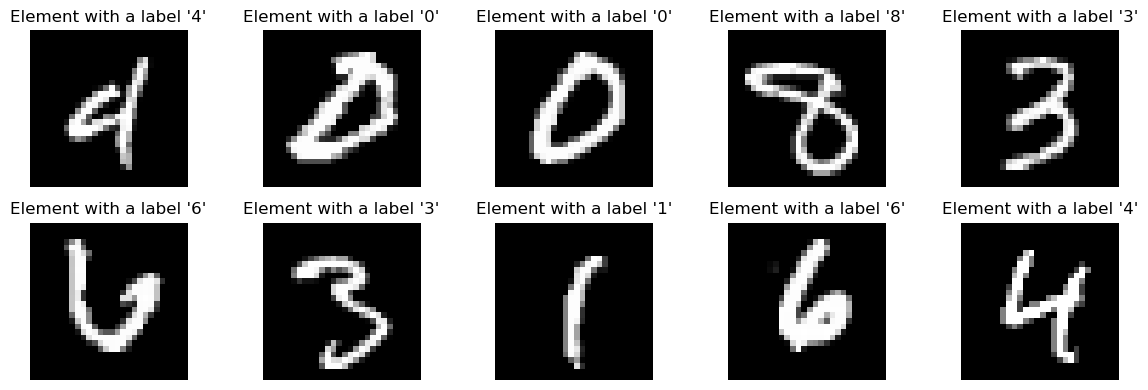
\includegraphics[width=\textwidth]{figures/dataset.png}
    \caption{Representative samples from the MNIST dataset \cite{lecun2010mnist} with their corresponding labels.}
    \label{mnist:fig}
\end{figure}

We approached the image classification task as a semi-supervised learning problem, training models on varying fractions of labeled training data (25\%, 50\%, 75\%, and 100\%). The training dataset was split using uniform sampling into labeled and unlabeled portions according to the specified percentages. For the Triplet Network, we employed a Convolutional Neural Network architecture consisting of two Convolutional Layers with 3x3 filters (feature map dimensions of 32 and 64, respectively, with $\text{stride}=1$ and $\text{padding}=1$), followed by 2x2 Max-Pooling layers, and two Dense Layers. ReLU non-differentiable activation functions were utilized throughout the network, introducing non-linearity to each layer. Together with non-smooth Triplet loss function this makes the learning problem highly non-smooth and non-convex (see discussion of this issue in \cite{Norkin_2021}). We trained separate Triplet Network models for each labeled data fraction with the following hyperparameters: 50 epochs, batch size of 1000, learning rate $\rho = 10^{-3}$, and $l_2$ regularization rate $\lambda = 10^{-5}$. For the triplet loss (\ref{triplet-loss-func:eq}) and triplet mining (\ref{semi-hard-triplet-mining:eq}), we set the margin hyperparameter $\alpha = 1.0$. To facilitate meaningful feature capture while enabling visualization, we chose a latent space $\mathbb{R}^3$ of dimensionality $n=3$. Fig.~\ref{latent-space:fig} gives latent representations of images in the train dataset (left) and test dataset (right) projected by the Triplet Network, with each element gray-coded according to its label (0-9). The clustering of elements with the same label suggests that the Triplet Network successfully captured relevant features during training.

\begin{figure}
    \centering
    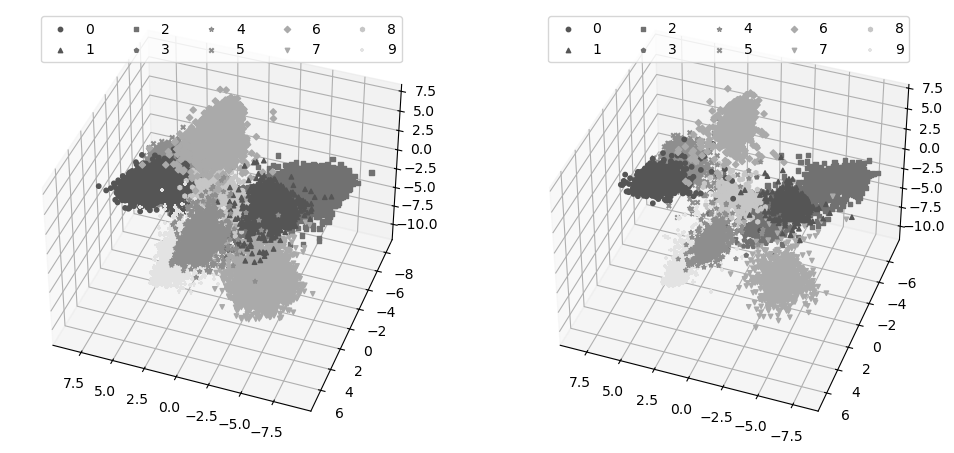
\includegraphics[width=\textwidth]{figures/latent_space.png}
    \caption{Latent representations of images in the train dataset (left) and test dataset (right) projected by the Triplet Network, with each element color-coded according to its label (0-9). The clustering of elements with the same label suggests that the Triplet Network successfully captured relevant features during training.}
    \label{latent-space:fig}
\end{figure}

\begin{figure}
    \centering
    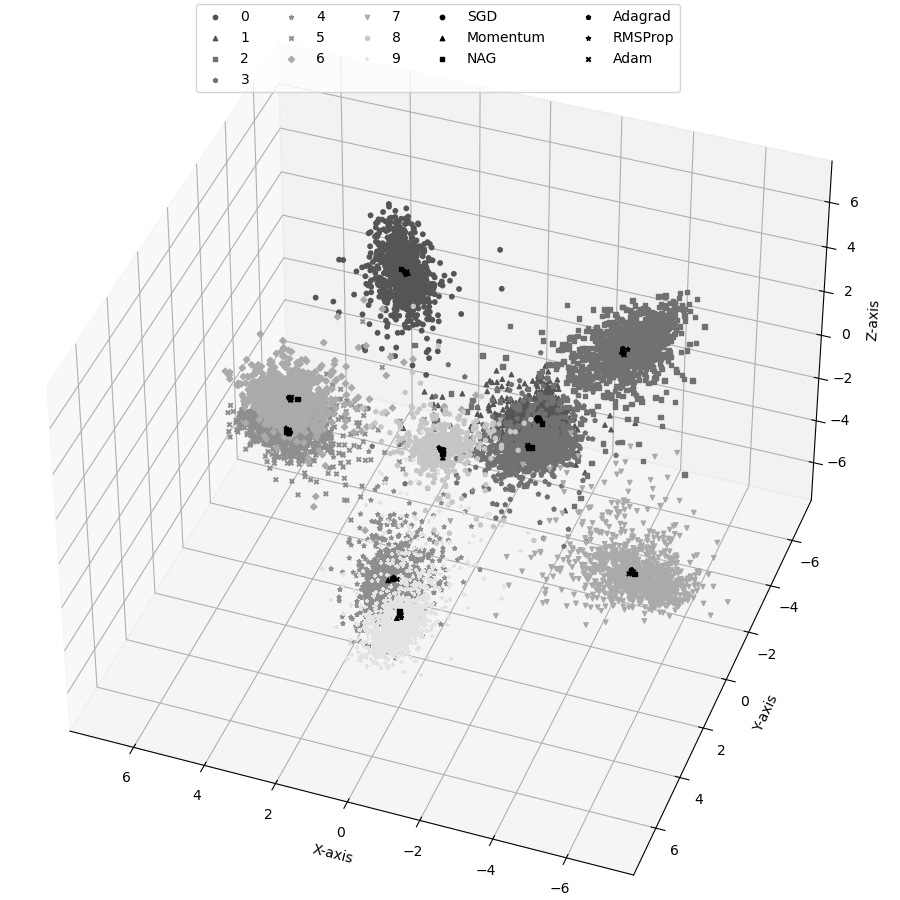
\includegraphics[width=0.8\textwidth]{figures/sq_quants.png}
    \caption{Optimal positions of quants for each Stochastic Quantization variant (labeled by variant name) in the latent space, relative to labeled elements (0-9) from the test dataset.}
    \label{quants:fig}
\end{figure}

The Triplet Network was used to project latent representations onto $\mathbb{R}^3$ space from both labeled and unlabeled training data. These representations were then used to train the Stochastic Quantization algorithm as an unsupervised learning model. For each set of latent representations corresponding to different labeled data fractions, we trained the Stochastic Quantization algorithm and its adaptive variants (\ref{momentum-update-rule:eq})-(\ref{adam-update-rule:eq}) from subsection \ref{adap-stoch-quant:sec}. The initialization strategy for quant positions utilized uniform sampling from a labeled data fraction for each label. To ensure convergence, we set the rank hyperparameter to $r = 3$ and employed different learning rates for each variant: $\rho = 0.001$ for SGD, Momentum, NAG, RMSProp; $\rho = 0.1$ for AdaGrad; and $\rho = 0.01$ for ADAM. With these hyperparameters, all Stochastic Quantization variants converged to the global optima. Fig.~\ref{quants:fig} shows optimal positions of quants for each Stochastic Quantization variant (labeled by variant name) in the latent space, relative to labeled elements (0-9) from the test dataset. Fig.~\ref{convergence:fig} presents a comparative analysis of the convergence rates for the Stochastic Quantization variants by plotting the objective function value (\ref{global-sq-fn-expansion:eq}) against the iteration number $t$.

\begin{figure}
    \centering
    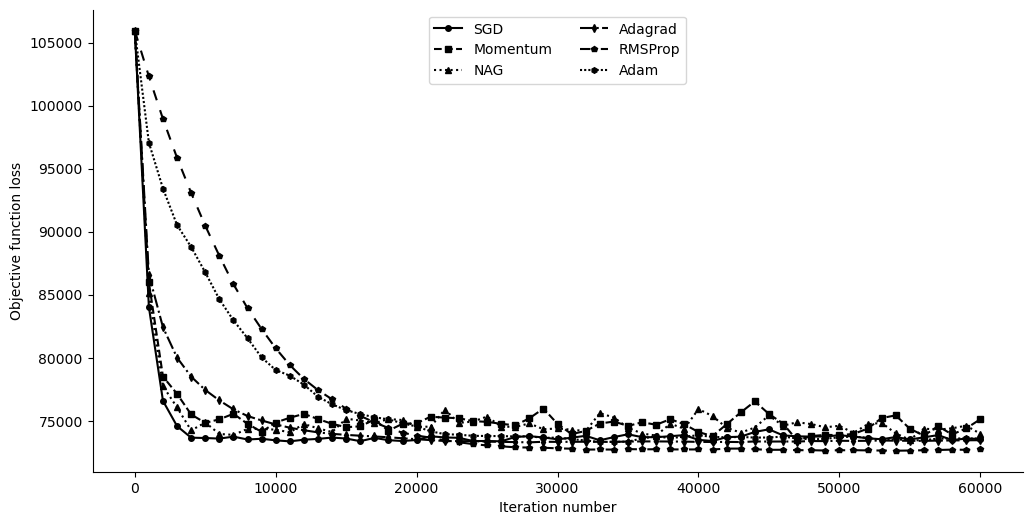
\includegraphics[width=\textwidth]{figures/convergence/sq_convergence_100.png}
    \caption{Convergence speed comparison of Stochastic Quantization variants on latent representations of training data with 100\% labeled fraction.}
    \label{convergence:fig}
\end{figure}

The accuracy of the trained classification models, combining Triplet Network and Stochastic Quantization, was evaluated using the F1-score metric \cite{Chinchor_1992} for weighted multi-label classification. Our experiments demonstrated that our approach achieved results comparable to state-of-the-art performance with Triplet Network and Siamese Network, as reported in \cite{Hoffer_2015}, even with limited labeled data. Table~\ref{accuracy:table} presents a comprehensive comparison of classification accuracy across different algorithms and percentages of training data.

\begin{table}
\caption{Classification accuracy comparison on MNIST dataset \cite{lecun2010mnist}.}
    \label{accuracy:table}
    \begin{tabularx}{\textwidth}{|X|*{4}{c|}}
        \hline
        \multirow{2}{*}{Algorithm} & \multicolumn{4}{c|}{Percentage of Training Data} \\
        \cline{2-5}
        & 25\% & 50\% & 75\% & 100\% \\
        \hline
        Triplet Network + KNN         &    -    &    -    &    -    & 99.54\% \\
        Siamese Network + KNN         &    -    &    -    &    -    & 97.90\% \\
        Triplet Network + SQ-SGD      & 78.10\% & 97.74\% & 97.83\% & 98.38\% \\
        Triplet Network + SQ-Momentum & 78.06\% & 97.73\% & 97.82\% & 98.36\% \\
        Triplet Network + SQ-NAG      & 78.00\% & 97.63\% & 97.72\% & 98.33\% \\
        Triplet Network + SQ-AdaGrad  & 78.95\% & 97.72\% & 97.79\% & 98.34\% \\
        Triplet Network + SQ-RMSProp  & 79.34\% & 97.70\% & 97.80\% & 98.29\% \\
        Triplet Network + SQ-ADAM     & 79.15\% & 97.70\% & 97.86\% & 98.29\% \\
        \hline
    \end{tabularx}
\end{table}
